\subsubsection{Strategiemodul} \label{sec:strategy}

Das Strategiemodul \texttt{strategy.pl} stellt das Prädikat zur Bestimmung des nächsten Angriffspunktes \texttt{getPointOfAttack/2}	zur Verfügung. 
Außerdem füllt dieses Modul die Liste der priorisiert anzugreifenden Punkte über das Prädikat \texttt{updateOpenList/3}. 

Beim Aufruf von \texttt{getPointOfAttack/2} wird das erste Element der Openlist \texttt{openList/2} zurückgegeben.
Befinden sich keine Koordinaten in der Openlist \texttt{openList/1}, so gibt \texttt{getPointOfAttack/2} einen zufälligen Angriffspunkt zurück.

Das Prädikat \texttt{updateOpenList/3} erhält die angegriffene Koordinate und den vom Gegner erhaltenen Rückgabewert. 
Traf der Angriff Wasser oder das letzte Schiff des Gegners, so wird lediglich die angegriffene Position aus der Openlist gelöscht.

Wurde das gerade attackierte Schiff vollständig versenkt, so kann die aktuelle Openlist vollständig geleert werden, da stets nur ein Schiff attackiert wird. 
Außerdem werden die unmittelbar benachbarten Felder des versenkten Schiffes als \textit{Wasser} markiert, denn aufgrund der Spielregeln darf sich auf diesen Feldern kein weiteres Schiff befinden (Prädikat \texttt{surroundWithWater/4}). 

Ist die Antwort des Gegeners \textit{Treffer}, so muss die Openlist aktualisiert werden. 
Dazu werden zunächst alle benachbarten Felder in die Openlist eingetragen, deren Status unbekannt ist (Prädikat \texttt{appendFreeFieldToList/2}). 

Als mögliche Kandidaten der Openlist gehen die Felder der direkten 4er-Nachbarschaft des Treffers ein, wie es in Abbildung \ref{fig:ErstelleOpenlist} zu sehen ist.
Die Reihenfolge wurde auf Westen, Osten, Norden, Süden festgelegt.
\begin{figure}[H]
  \centering
  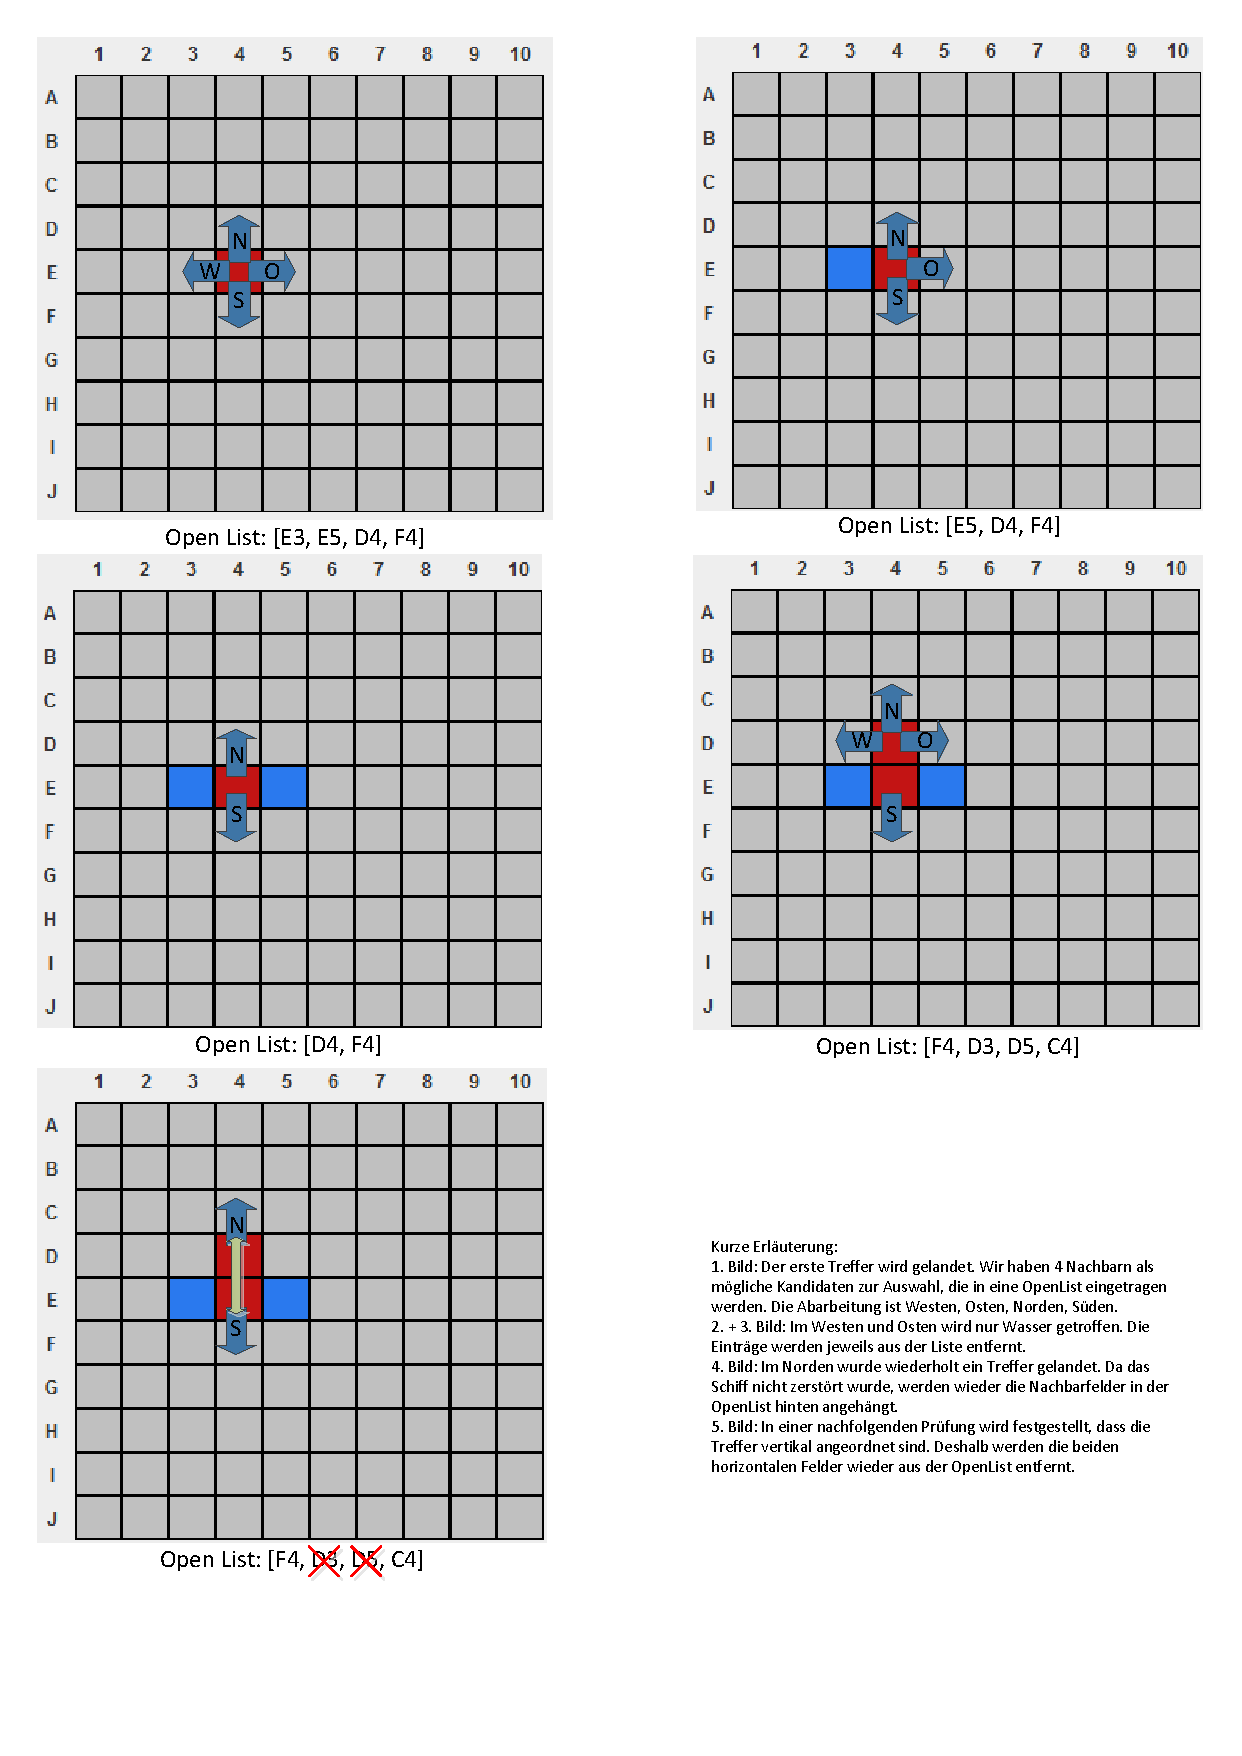
\includegraphics[trim=5mm 204mm 105mm 4mm,clip,width=0.5\textwidth]{images/Strategie_1_FirstHit.pdf}
  \caption{Openlist mit benachbarten Feldern initialisieren}
  \label{fig:ErstelleOpenlist}
\end{figure}

In den nachfolgenden Spielzügen werden diese Felder geprüft.
Sollten diese sich als "'Wasser"' herausstellen, wie es in der Abbildung \ref{fig:Openlist2} angedeutet ist, so werden die entsprechenden Einträge ohne weitere Verarbeitung aus der Openlist gelöscht.
\begin{figure}[H]
  \centering
  \subfigure[Westen (verfehlt)]{
    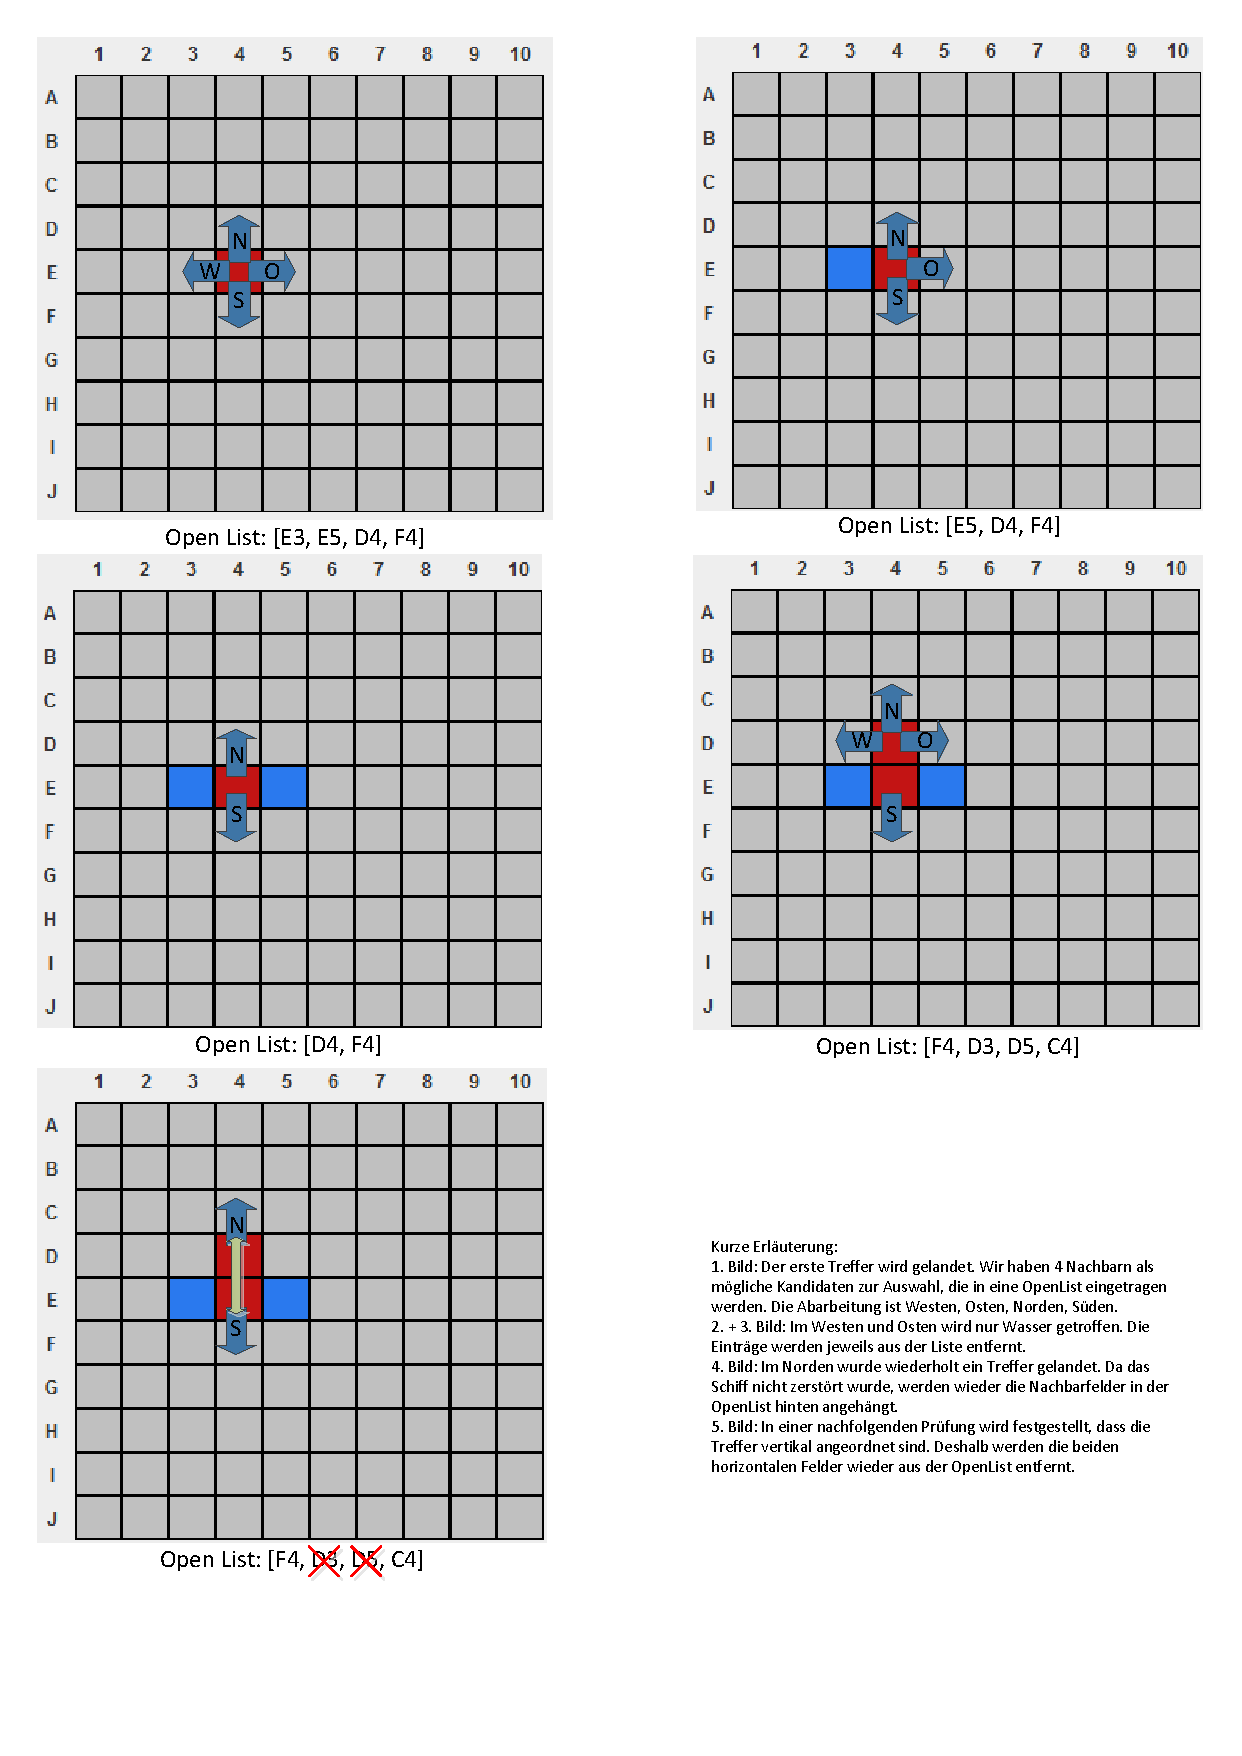
\includegraphics[trim=105mm 204mm 5mm 4mm,clip,width=0.47\textwidth]{images/Strategie_1_FirstHit.pdf}
    \label{fig:west}
  }
  \subfigure[Osten (verfehlt)]{
	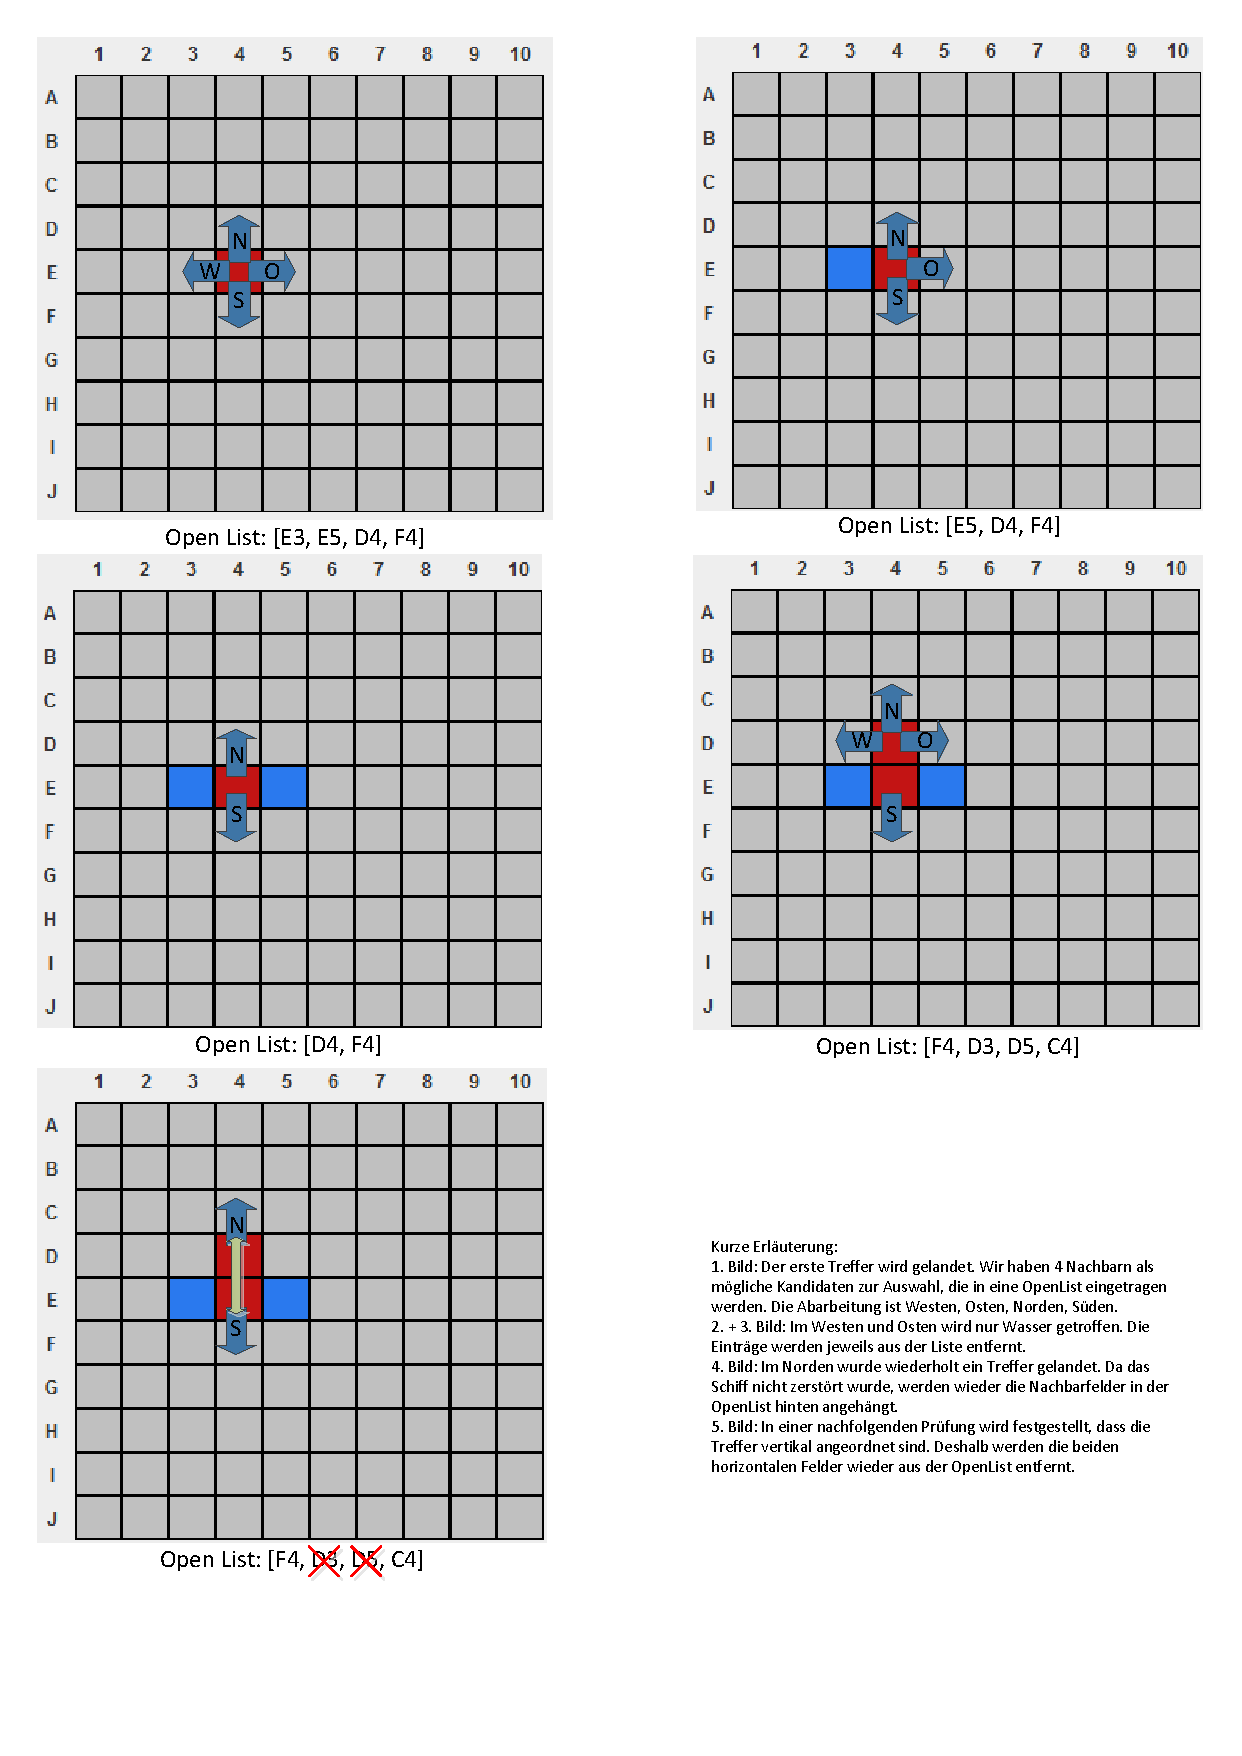
\includegraphics[trim=5mm 117mm 105mm 94mm,clip,width=0.47\textwidth]{images/Strategie_1_FirstHit.pdf}
    \label{fig:east}
  }
  \caption{Openlist nach zwei misglückten Angriffen}
  \label{fig:Openlist2}
\end{figure}

Im Falle eines weiteren Treffers wiederholt sich der Algorithmus und nimmt alle unbekannten und benachbarten Felder des Treffers in die Openlist auf (vgl. Abbilidung \ref{fig:north}).
Anschließend wird mit dem Prädikat \texttt{checkHitDirection/2} überprüft, ob die Orientierung des attackierten Schiffes (horizontal oder vertikal) bereits durch frühere Treffer bekannt ist. 
Ist dies der Fall, so kann die Openlist entsprechend um auszuschließende Positionen verkürzt werden.
Im hier gezeigten Beispiel können die horizontalen Felder $D3$ und $D5$ wieder aus der Liste gestrichen werden.
\begin{figure}[H]
  \centering
  \subfigure[Norden (Treffer)]{
    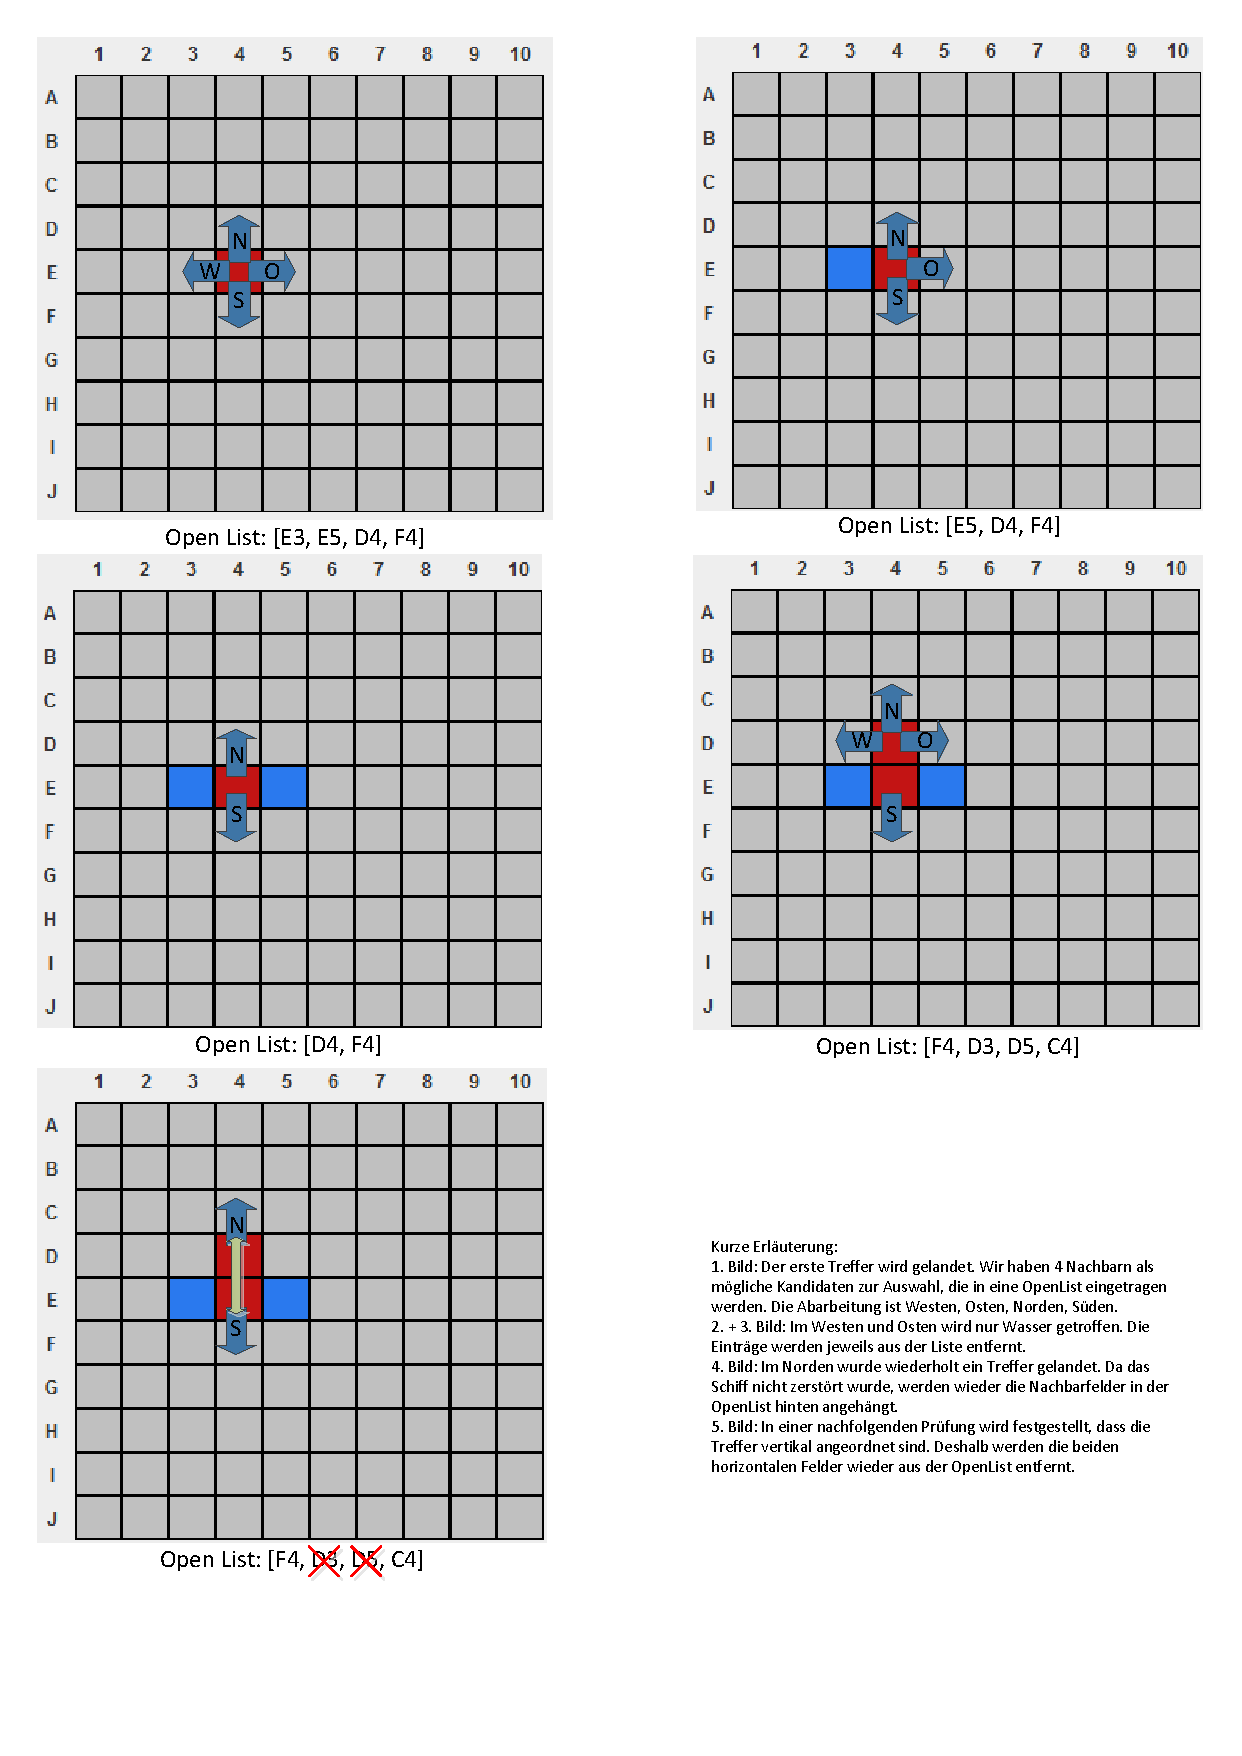
\includegraphics[trim=105mm 117mm 5mm 94mm,clip,width=0.47\textwidth]{images/Strategie_1_FirstHit.pdf}
    \label{fig:north}
  }
  \subfigure[Bereinigte Openlist]{
	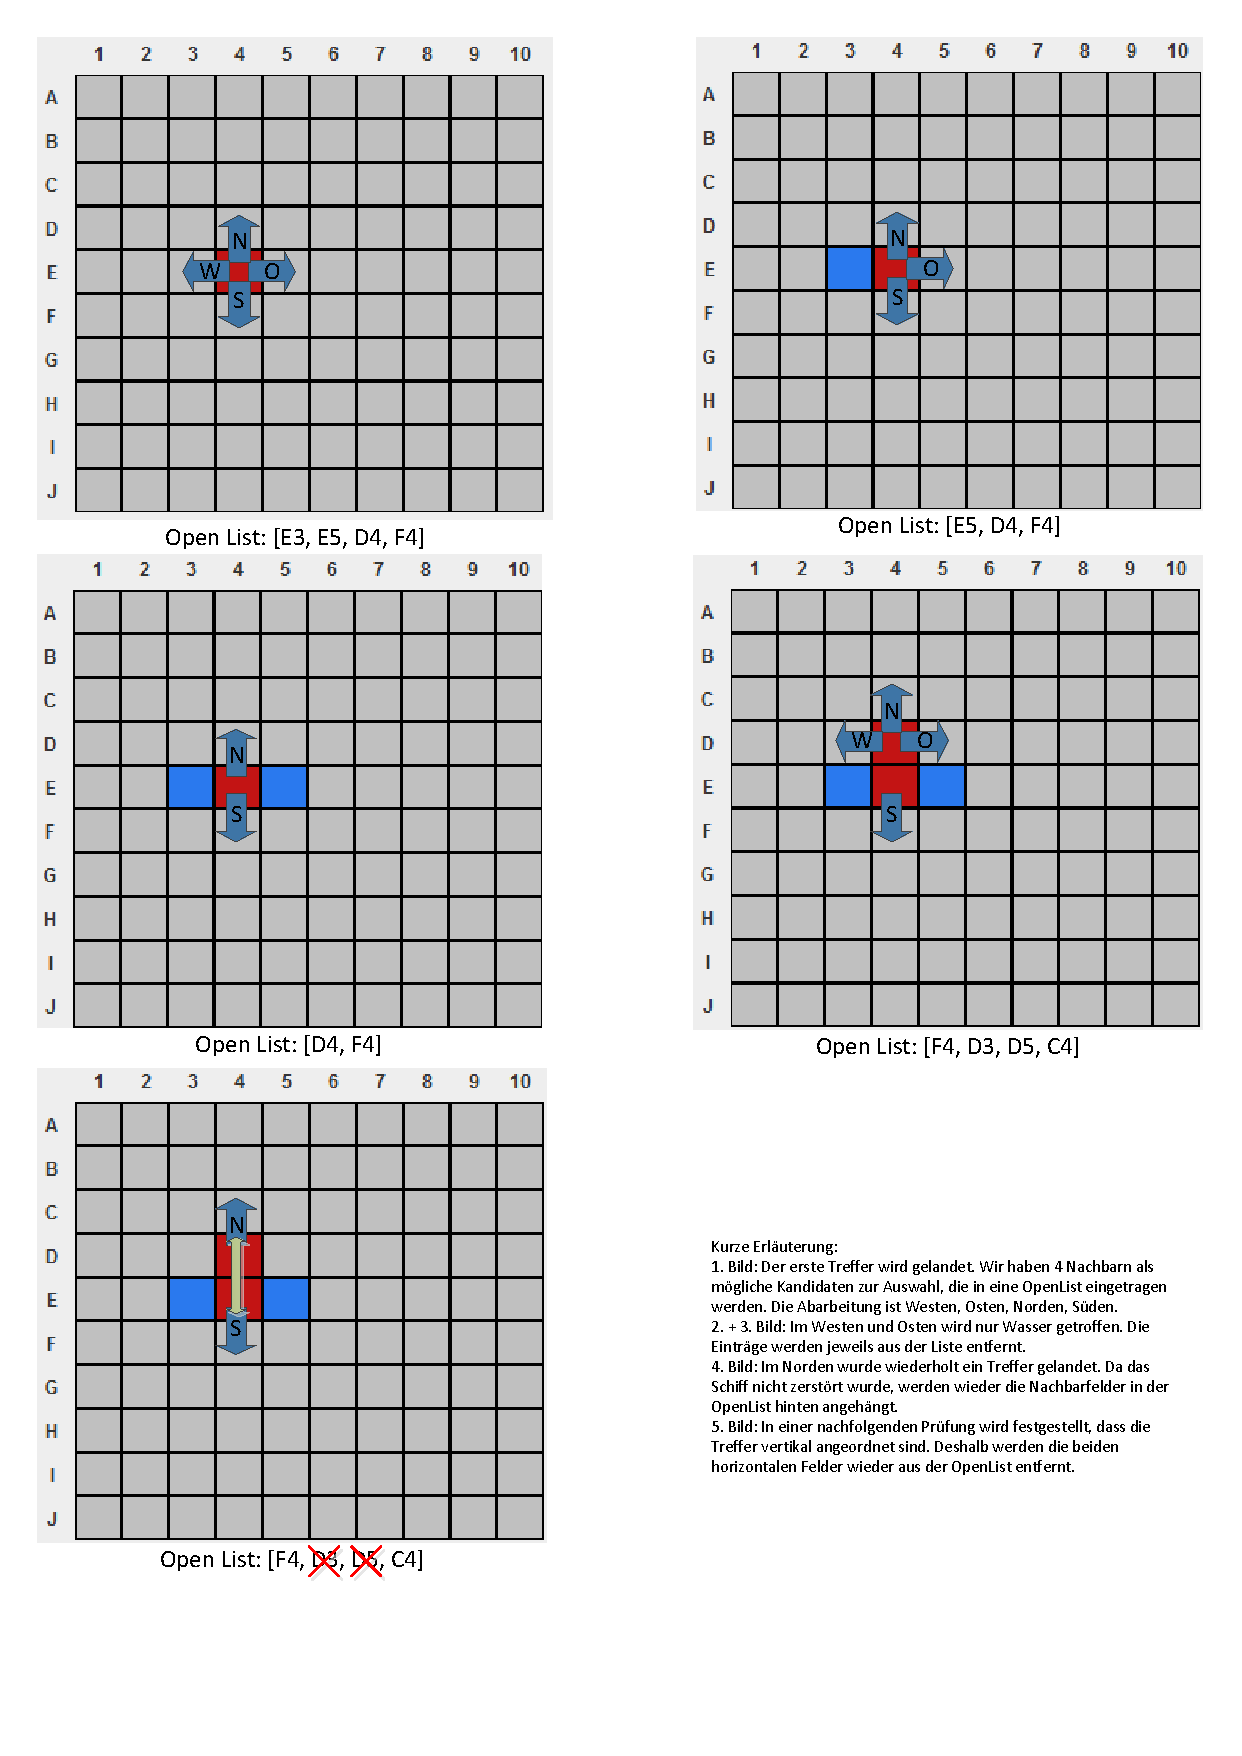
\includegraphics[trim=5mm 30mm 105mm 180mm,clip,width=0.47\textwidth]{images/Strategie_1_FirstHit.pdf}
    \label{fig:northupd}
  }
  \caption{Aktualisierung der Openlist nach einem Treffer}
  \label{fig:Openlist3}
\end{figure}

Nachdem das Schiff vollständig zerstört wurde, wird die Openlist geleert und die Auswahl der anzugreifenden Koordinaten erfolgt wieder solange zufällig, bis der nächste Treffer erzielt wurde.